\documentclass{beamer}
\usepackage{graphicx}
\usepackage{booktabs}
\usepackage{hyperref}
\usepackage{comment}
\usetheme{Madrid}

\title[]{Cumulative No Reasoning with Large Language Models}
\subtitle{by Yifan Zhang, Jingqin Yang, Yang Yuan, Andrew Chi-Chih Yao}
\author{Peer Niklas Schäfer}
\institute{University of Cologne}
\date{18.06.2025}

\begin{document}

\begin{frame}
    \titlepage
\end{frame}

%-------------------------------

\begin{frame}{}
    \begin{center}
        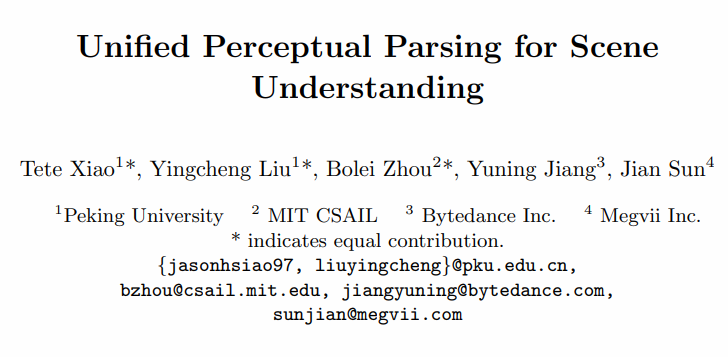
\includegraphics[width=0.8\linewidth]{Images/paper.png}

        \tiny{26 Jul 2018}
    \end{center}
\end{frame}

%-------------------------------

\begin{frame}{What is Unified Perceptual Parsing?}
    \begin{itemize}
        \item Humans perceive a scene by identifying:
        \begin{itemize}
            \item Scene type (e.g., kitchen)
            \item Objects (e.g., stove, table)
            \item Objects parts (e.g., table leg, stove knob)
            \item Materials (metal, wood)
            \item Textures (smooth, rough)
        \end{itemize}
        \item \textbf{Unified Perceptual Parsing} aims to do all this with a single model.
    \end{itemize}
    \vfill
    \begin{center}
        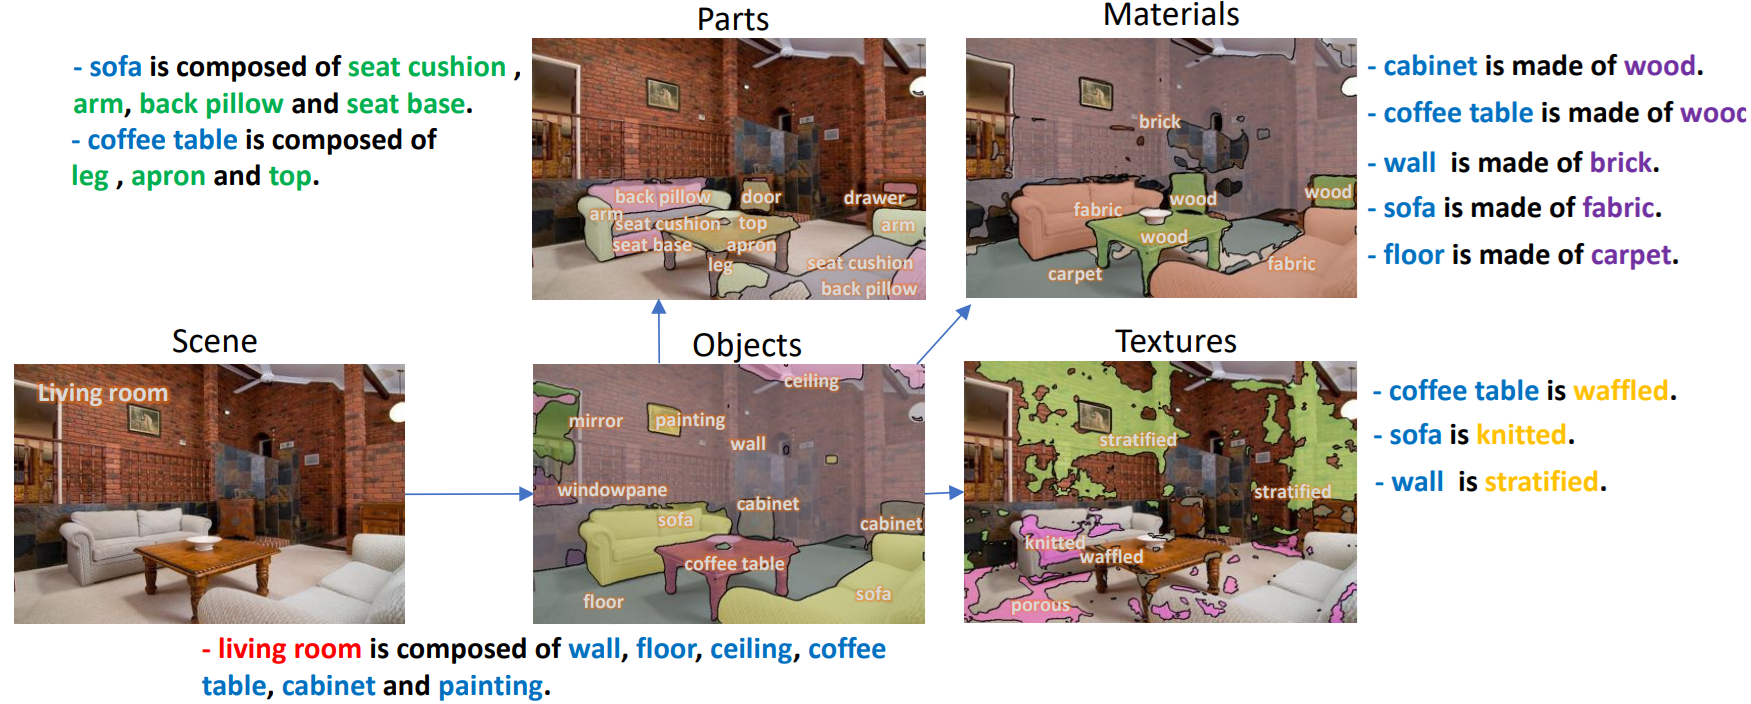
\includegraphics[width=0.8\linewidth]{Images/intro_segmentation.png}
    \end{center}
\end{frame}

%-------------------------------

\begin{frame}{Why Is This Challenging?}
  \begin{itemize}
    \item Perceptual parsing combines very different tasks:
    \begin{itemize}
      \item Scene classification (high-level understanding)
      \item Object and part segmentation (mid-level)
      \item Material and texture recognition (low-level, detailed)
    \end{itemize}

    \vspace{0.3cm}

    \item These tasks vary in:
    \begin{itemize}
      \item The type of information they require
      \item Spatial scale and detail level
    \end{itemize}

    \vspace{0.3cm}

    \item \textbf{Challenge:} One model must handle all levels — from big picture to fine details.
  \end{itemize}
\end{frame}

%-------------------------------

\begin{frame}{Previous Work}
  \begin{itemize}
    \item \textbf{Scene Classification:} CNNs like ResNet, trained on datasets like Places
    \item \textbf{Semantic Segmentation:} FCN, DeepLab (object-level)
    \item \textbf{Part Segmentation:} Pascal-Parts
    \item \textbf{Material / Texture:} OpenSurfaces, DTD
  \end{itemize}
  
  \vspace{0.4cm}
  
  \begin{block}{Before This Paper}
    \begin{itemize}
      \item Each task was handled by a separate model
      \item No feature sharing between tasks
      \item Training and inference were inefficient and fragmented
    \end{itemize}
  \end{block}
\end{frame}

%-------------------------------

\begin{frame}{Main Contribution of This Paper}
  \textbf{Objective:} Develop a single unified network for parsing multiple semantic levels from one image.

  \vspace{0.5cm}

  \begin{itemize}
    \item Create \textbf{Broden+} – unified dataset from various sources
    \item Propose \textbf{UPerNet} – a multi-task network on top of FPN
    \item Define a \textbf{joint benchmark} for perceptual parsing
  \end{itemize}

  \vfill
  \textit{One image in, multiple perceptual layers out.}
\end{frame}

%-------------------------------

\begin{frame}{What is Broden+?}
  \begin{itemize}
    \item \textbf{Broden+} is a large-scale, unified dataset built by merging:
    \begin{itemize}
      \item ADE20K: Scene and object segmentation
      \item Pascal-Context: Part segmentation
      \item OpenSurfaces: Material labels
      \item DTD (Describable Textures Dataset): Texture attributes
    \end{itemize}
    \item Provides a \textbf{diverse set of annotations} per image:
    \begin{itemize}
      \item Scene labels, object masks, parts, textures, materials
    \end{itemize}
  \end{itemize}
  \vfill
  \textit{Goal: Combine multiple visual concepts in a single dataset.}
\end{frame}

\begin{frame}{Why Was Broden+ Manually Merged?}
  \textbf{No single existing dataset} had all the annotations needed for unified perceptual parsing.

  \vspace{0.4cm}

  \textbf{Limitations of existing datasets:}
  \begin{itemize}
    \item Each focuses on \textbf{only one or two tasks} (e.g., objects OR textures)
    \item Different label sets, formats, and definitions
    \item No shared vocabulary across datasets
  \end{itemize}

  \vspace{0.4cm}

  \textbf{Manual merging needed to:}
  \begin{itemize}
    \item \textbf{Standardize labels and semantics} across tasks
    \item Ensure \textbf{consistent pixel-level quality}
    \item Enable multi-task supervision in a unified setting
  \end{itemize}
\end{frame}

\begin{frame}{How Was Broden+ Merged?}
  
  \textbf{Merging Criteria:}
  \begin{itemize}
    \item All annotations are \textbf{mapped to a shared vocabulary}
    \item Images are labeled with \textbf{as many tasks as possible}
    \item Only high-quality, pixel-aligned annotations are kept
    \item Some rare classes were \textbf{merged into broader categories} to reduce noise and improve consistency (stone and concrete are merged into stone)
  \end{itemize}
\end{frame}

\begin{frame}{Friedhof}

\end{frame}

%-------------------------------

\begin{frame}{How Was Broden+ Merged?}
  \begin{center}
    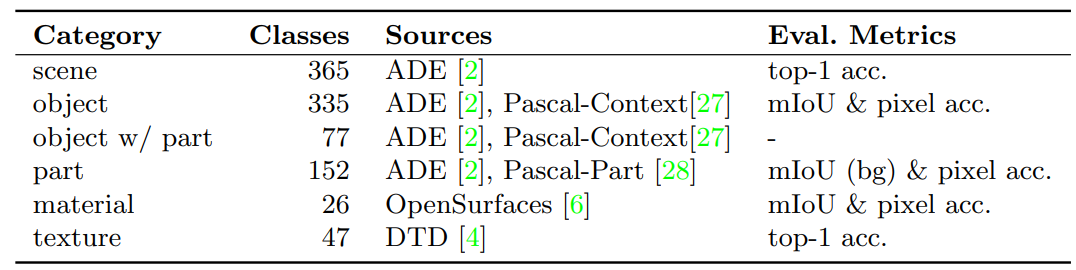
\includegraphics[width=0.8\linewidth]{Images/BrodenDataset.png}
    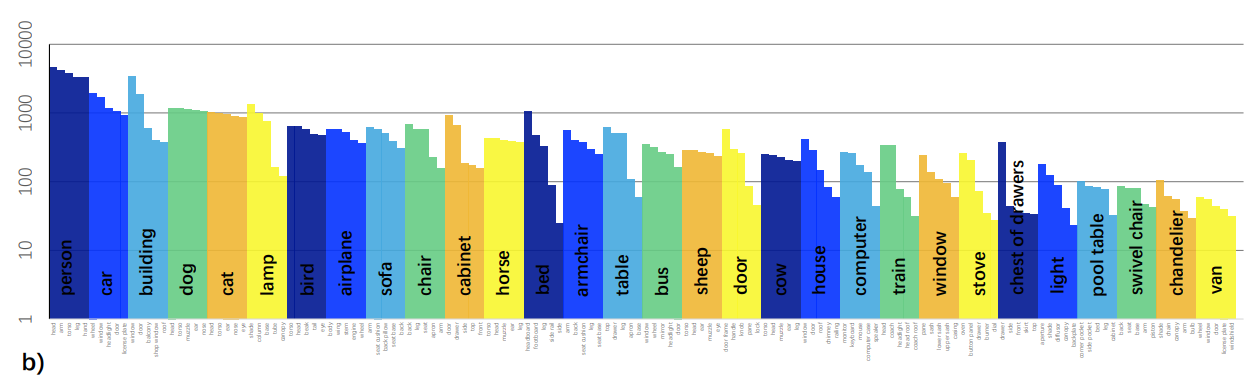
\includegraphics[width=0.8\linewidth]{Images/ObjectClasses.png}
  \end{center}
\end{frame}

%-------------------------------

\begin{frame}{How Is Performance Measured?}
  \vspace{0.4cm}
  \begin{tabular}{ll}
    \textbf{Task} & \textbf{Metric} \\
    \hline
    Scene Classification & Top-1 Accuracy \\
    Object Segmentation & Mean IoU (Intersection over Union) \\
    Part Segmentation & Mean IoU \\
    Material Prediction & Pixel Accuracy \\
    Texture Prediction & Image-level Classification Accuracy \\
  \end{tabular}
  \vspace{0.5cm}
  \begin{itemize}
    \item Evaluated on the unified benchmark created from \textbf{Broden+}.
    \item \textbf{Multi-task setting:} All tasks evaluated using a shared backbone and features.
  \end{itemize}
  \vfill
  \textit{Goal: Assess how well the unified model performs across diverse visual tasks.}
\end{frame}

\end{document}
